\documentclass[8pt]{beamer}

\usetheme{Darmstadt}
\usecolortheme{dove}
\usepackage[small,center]{caption}
\usepackage{times}
\usefonttheme{structurebold}
\usepackage[english]{babel}
\usepackage{pgf,pgfarrows,pgfnodes,pgfautomata,pgfheaps}
\usepackage{amsmath,amssymb}
\usepackage{amsxtra}

\usepackage{caption}
\usepackage{tikz}
\usetikzlibrary{shapes.misc}

\newcommand{\leftd}[1]{{\color{red} \bar{#1}}}
\newcommand{\interface}[2]{{\color{blue}{#1}_I(#2)}}
\newcommand{\leftdd}[2]{{\color{red} \bar{#1}(\bar{#2})}}
\newcommand{\leftFourier}[1]{{\color{red} \hat{#1}}}
\newcommand{\leftFourierTwo}[2]{{\color{red} \hat{#1}(\hat{#2})}}
\newcommand{\divergence}{\mathrm{div}}

\newcommand{\I}{I}

\newcommand*{\vcenterimage}[1]{\vcenter{\hbox{\includegraphics[width=2in]{#1}}}}
\newcommand*{\vcenterarrow}{\vcenter{\hbox{$\Longrightarrow$}}}

\newcommand{\euleriandx}{{\ensuremath{\Delta x}}}
\newcommand{\half}{{\ensuremath{\frac{1}{2}}}}
\newcommand{\Chib}{\boldsymbol{\chi}}
\newcommand{\xface}{{i + \half, j, k}}
\newcommand{\xb}{\boldsymbol{x}}
\newcommand{\Xb}{\boldsymbol{X}}

\DeclareMathOperator{\hyphen}{-}

\definecolor{Carolinablue}{RGB}{75, 156, 211}
\definecolor{ballblue}{rgb}{0.13, 0.67, 0.8}
\definecolor{lightgray}{rgb}{0.83, 0.83, 0.83}
\setbeamercolor{block title}{bg=lightgray,fg=Carolinablue}
\setbeamercolor{block body}{bg=white,fg=black}
\setbeamercovered{dynamic}
\setbeamercolor*{item}{fg=Carolinablue}

\captionsetup[subfigure]{labelformat=empty}
\captionsetup[figure]{labelformat=empty}
\setbeamertemplate{navigation symbols}{}
\setbeamertemplate{footline}[frame number]
\begin{document}

% tikz stuff
\tikzset{cross/.style={cross out, draw=black, minimum size=2*(#1-\pgflinewidth),
inner sep=0pt, outer sep=0pt},
%default radius will be 1pt.
cross/.default={2.5pt}}

%% What is great about PETSc? I'm on the outside and I'm looking in
%%
%% 1. From the deal.II developer meeting on May 16: getting all warnings on all
%%    platforms fixed is really hard. We can't afford to run our full test suite
%%    on every PR. PETSc's CI is awesome!
%%
%% 2. From a CI run on May 17: ran 4728 tests in 56 minutes. We can barely compile
%%    deal.II in 56 minutes :(
%%
%% 3. From another recent CI run (10066447923);
%%
%%    # -------------
%%    #   Summary
%%    # -------------
%%    # success 11314/11314 tests (100.0%)
%%    # failed 0/11314 tests (0.0%)
%%    # todo 0/11314 tests (0.0%)
%%    # skip 0/11314 tests (0.0%)
%%    #
%%    # Wall clock time for tests: 1490 sec
%%    # Approximate CPU time (not incl. build time): 4778.100000000056 sec
%%
%%    very impressive throughput!
%%
%% 4. Incremental builds are basically instantaneous (deal.II is a lot better at
%%    this now that the mold linker exists)
%%
%% 5. Installing dependencies is hard - BuildSystem's --download-XYZ saves me a
%%    huge amount of time and effort (thanks!); we use it with autoibamr
%%
%% 6. Somewhat ineffable: clearly a project written by people who care and have
%%    a consistent vision
%%
%% How does IBAMR use PETSc? What have we accomplished over the last six years?
%%
%% 1. INS solver. Show an example run script. Very exciting that Mats and Vecs
%%    work with data from libMesh, deal.II, or SAMRAI!
%%
%% 2. Velocity interpolation: Whatever we did to avoid VecStash. Note that our
%%    needs are past what I know how to accomplish with libMesh - we moved on to
%%    a (not publicly available) deal.II implementation
%%
%%    a. Velocity interpolation looks like setting up a load vector: we're doing
%%       an L2 projection which samples the velocities on the Cartesian grid at
%%       known quadrature points.
%%
%%    b. Added difficulty: just because a Patch is locally owned doesn't mean that
%%       the elements which intersect it are!
%%
%% 3. Force spreading: SAMRAIGhostDataAccumulator (uses both indexing and summation)
%%    First part: we want to do fast array access, so we need local DoFs. How do
%%    we get that in a finite difference context (where we normally don't even
%%    bother assigning DoFs)?
%%
%%    a. In IBAMR there are O(nproc) patches and their structure is known on all
%%       processors: relatively easy to get a global enumeration DoFs with purely
%%       SAMRAI stuff
%%
%%    b. Set all indices we don't need to `-1` (e.g., ghost cells outside the
%%       physical domain)
%%
%%    c. Use local and ghost DoFs to make a `VECGHOST'
%%
%%    d. Use `VecGetLocalToGlobalMapping()` + `ISGlobalToLocalMappingApply()`: we
%%       now have all local DoF indices (fast!)
%%
%%    Now we have local indices - we can just use `VecGhostGetLocalForm()` and
%%   `VecSetValues()` (and `VecGhsotRestoreLocalForm()`) and that's enough!

\frame{
\title{\Large IBAMR: Immersed-Boundary Adaptive Mesh Refinement}

\author{{\Large David Wells \\\vspace{0.1in} University of North Carolina}    \\
\vspace{0.2in} {Cardiovascular Modeling and Simulation Lab}}

\date{May 20, 2025\\{}}

\begin{figure}[h]
\centering

\includegraphics[width=1.5in]{UNC_logo_542.eps}
 \end{figure}%

\vspace{-0.2in}
\titlepage
}

\section{Background}
\begin{frame}
    \frametitle{Collaborators}
    \begin{itemize}
    \item[$\blacksquare$] Laryssa Abdala, Bryn Barker, Cole Gruninger, Marshall Davey, Boyce Griffith (UNC)
    \item[$\blacksquare$] Charles Puelz (University of Houston)
    \item[$\blacksquare$] Amneet Bhalla (San Diego State University)
    \item[$\blacksquare$] deal.II supports tetrahedra! (Peter Munch, Technical University of Berlin)
    \end{itemize}
\end{frame}

\begin{frame}
    \frametitle{Content}
    \begin{itemize}
    \item[$\blacksquare$] Background
    \item[$\blacksquare$] Why use PETSc?
    \item[$\blacksquare$] Relevant Equations
    \item[$\blacksquare$] Fluid-Structure Interaction
    \item[$\blacksquare$] Where do we use PETSc?
    \item[$\blacksquare$] Future work (help me with \texttt{PCPATCH})
    \end{itemize}
\end{frame}

\begin{frame}
    \frametitle{Goals}
    \begin{itemize}
        \item[$\blacksquare$] On Alex's scale, I am mostly an HPC software
          developer and sometimes an applied mathematician
        \item[$\blacksquare$] I succeed when people can use my stuff to do
          cool things (like swimmers!)
        \item[$\blacksquare$] Principal developer of deal.II and IBAMR
        \item[$\blacksquare$] I've succeeded if I run out of time, not slides
          (feel free argue with me)
    \end{itemize}
\end{frame}

\begin{frame}
    \frametitle{Motivation}
    \begin{figure}
        \centering
        
\includegraphics[width=2in]{diagram-of-the-human-heart.pdf}
    \end{figure}
    \begin{itemize}
        \item[$\blacksquare$] 300,000 valve replacement surgeries each year - surgeons
          need more data
        \item[$\blacksquare$] Accurate multiphysics simulations of the cardiac cycle
        \item[$\blacksquare$] electrophysiology plus mechanics (Abdala), parallel
          scalability (Davey, Griffith, others), students write plugins, not monoliths (Cardinal)
    \end{itemize}
\end{frame}

\begin{frame}
    \frametitle{Incompressible fluids, hyperelastic incompressible structures}
    \begin{figure}
        \centering
        %% TODO: time permitting update this picture - we have better
        %% papilary muscles nowadays
        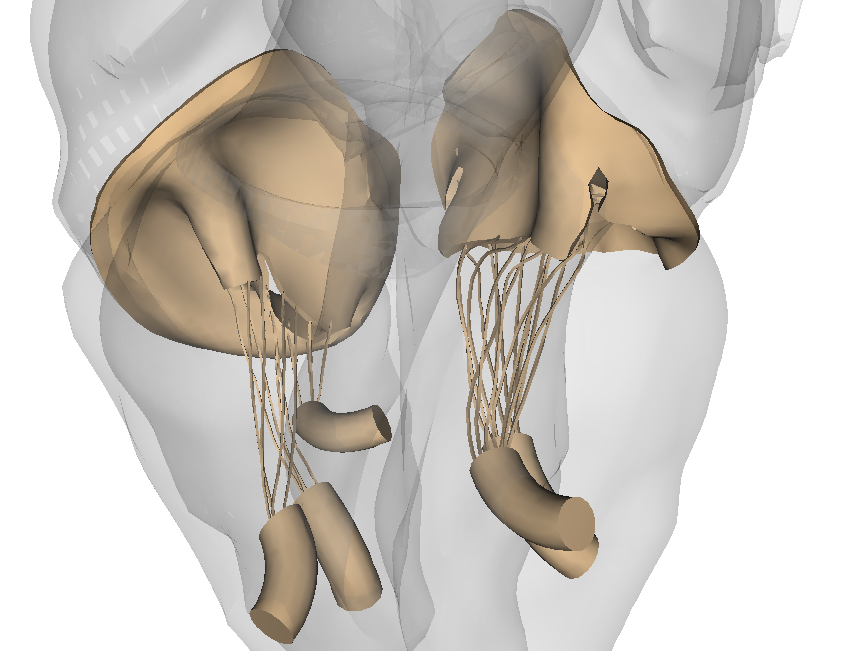
\includegraphics[width=2in]{mv_tv_front0037.png}
    \end{figure}
    \begin{itemize}
        \item[$\blacksquare$] Navier-Stokes: finite differences on a Cartesian grid
        \item[$\blacksquare$] Finite strain elasticity: finite elements on an
        unstructured mesh (libMesh or deal.II)
        \item[$\blacksquare$] Coupled with the immersed boundary (IB) method
    \end{itemize}
    The fluid and structure are assumed to have equal densities (neutral
    buoyancy).
\end{frame}

\begin{frame}
    \frametitle{Glossary}
        \vfill
    \begin{itemize}
        \item[$\blacksquare$] \emph{IBAMR}: Immersed Boundary Adaptive Mesh
        Refinement (software package at UNC; collaborators at SDSU, SUNY
        Buffalo, NWU, etc.) \texttt{https://www.github.com/IBAMR/IBAMR}
        \vfill
        \item[$\blacksquare$] \emph{deal.II}: Differential Equations Analysis
          Library, Version 2, (SIAM/ACM CSE Prize 2025)
          \texttt{https://www.dealii.org}
        \vfill
        \item[$\blacksquare$] \emph{Cell}: One cell in the Eulerian grid
        (managed by SAMRAI)
        \vfill
        \item[$\blacksquare$] \emph{Patch/Box}: A collection of Eulerian cells
        (between \(8x8x8\) and \(512x512x512\)) owned by one processor
        \vfill
        \item[$\blacksquare$] \emph{Element}: One element in (managed by
        libMesh or deal.II) one of the structures
        \vfill
        \item[$\blacksquare$] \emph{Quadrature Point}: Point for numerical
        integration. Points at which we couple the fluid and structure.
    \end{itemize}
        \vfill
\end{frame}

\section{Why Use PETSc?}

\begin{frame}[fragile]
    \frametitle{What is great about PETSc?}
    \begin{itemize}
      \item[$\blacksquare$] \emph{Stability}: Favors evolution over revolution (big problems with dealinos)
        \begin{center}
          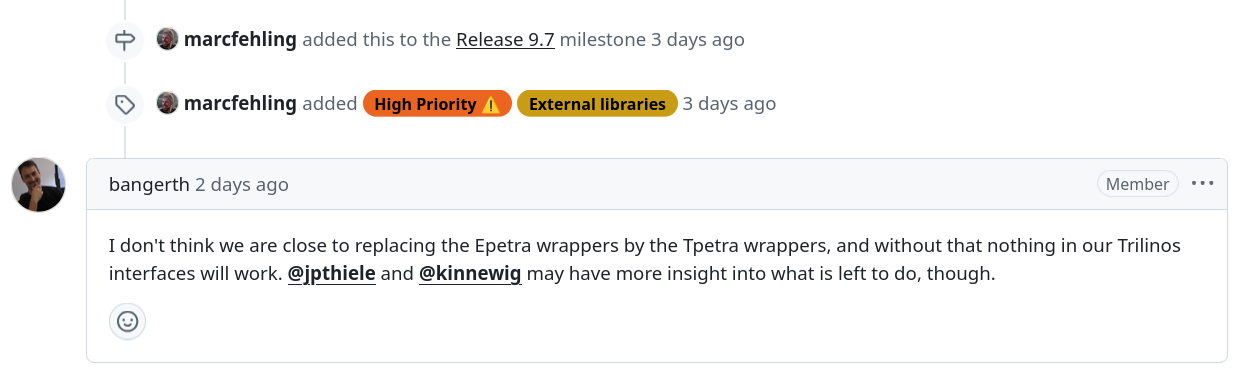
\includegraphics[width=4in]{tpetra.png}
        \end{center}
        \vfill

        \item[$\blacksquare$] \emph{BuildSystem}: consistently and correctly
          install dependencies in autoibamr:
\begin{verbatim}
for external_pkg in openblas hypre metis parmetis; do
    CONFOPTS="${CONFOPTS} --download-${external_pkg}=1"
done
\end{verbatim}
          Sometimes has problems with Python upgrades (XDR, Cython)
          \vfill

        \item[$\blacksquare$] \emph{Compatibility}: portable, no weird problems
          when \texttt{MPI\_Comm} is \texttt{unsigned int}
          \vfill
    \end{itemize}
\end{frame}

\begin{frame}[fragile]
    \frametitle{What does PETSc do exceptionally well?}
    \vfill
    \begin{itemize}
        \item[$\blacksquare$] \emph{Speed}: Recompilation is very fast,
          incremental builds, linking are nearly instantaneous. From a build in
          May:
\begin{verbatim}
%%    # -------------
%%    #   Summary
%%    # -------------
%%    # success 11314/11314 tests (100.0%)
%%    # failed 0/11314 tests (0.0%)
%%    # todo 0/11314 tests (0.0%)
%%    # skip 0/11314 tests (0.0%)
%%    #
%%    # Wall clock time for tests: 1490 sec
%%    # Approximate CPU time (not incl. build time): 4778.1 sec
\end{verbatim}
          \vfill
        \item[$\blacksquare$] \emph{Ineffability}: clearly a project written
          by people who care
          \vfill
        \item[$\blacksquare$] \emph{Just Works}: Get deal.II on the GPU via
          \texttt{VecSetType(v, VECKOKKOS)} and \texttt{MatSetType(m, MATKOKKOS)}
          (\texttt{dealii::MatrixFree} with Kokkos is WIP)
    \end{itemize}
    \vfill
\end{frame}

\section{Relevant Equations}
\begin{frame}
    \frametitle{Marker and Cell (MAC) scheme for incompressible flow}
    \begin{figure}
        \centering
        
\includegraphics[width=2in]{face-centered.pdf}
    \end{figure}
    \begin{itemize}
        \item[$\blacksquare$] An oldie, but a goodie (LANL 1965)
        \item[$\blacksquare$] Staggered discretization: face-centered
          velocities, cell-centered pressure
        \item[$\blacksquare$] Much better (10-100x) volume conservation (for
          structures) than collocated differences
        \item[$\blacksquare$] \emph{WIP}: SPD hanging nodes and higher order
          via Galerkin Differences (Barker)
    \end{itemize}
\end{frame}

\begin{frame}
    \frametitle{Fluid discretization with SAMR}
    \begin{figure}
        
\includegraphics[width=2in]{valid-grid-3-levels.pdf}
    \end{figure}
    \begin{itemize}
        \item[$\blacksquare$] \textbf{S}tructured \textbf{A}daptive \textbf{M}esh \textbf{R}efinement
        \item[$\blacksquare$] Finite differences on Cartesian grids: fast solvers
        \item[$\blacksquare$] Fine cells placed on structures and near important
        flow features
        \item[$\blacksquare$] Boundary conditions: simplified circuit-like
        models of the human body, do-nothing BC away from structure
    \end{itemize}
\end{frame}

\begin{frame}
    \frametitle{Finite element approximation of elastic structures}
    \begin{figure}
        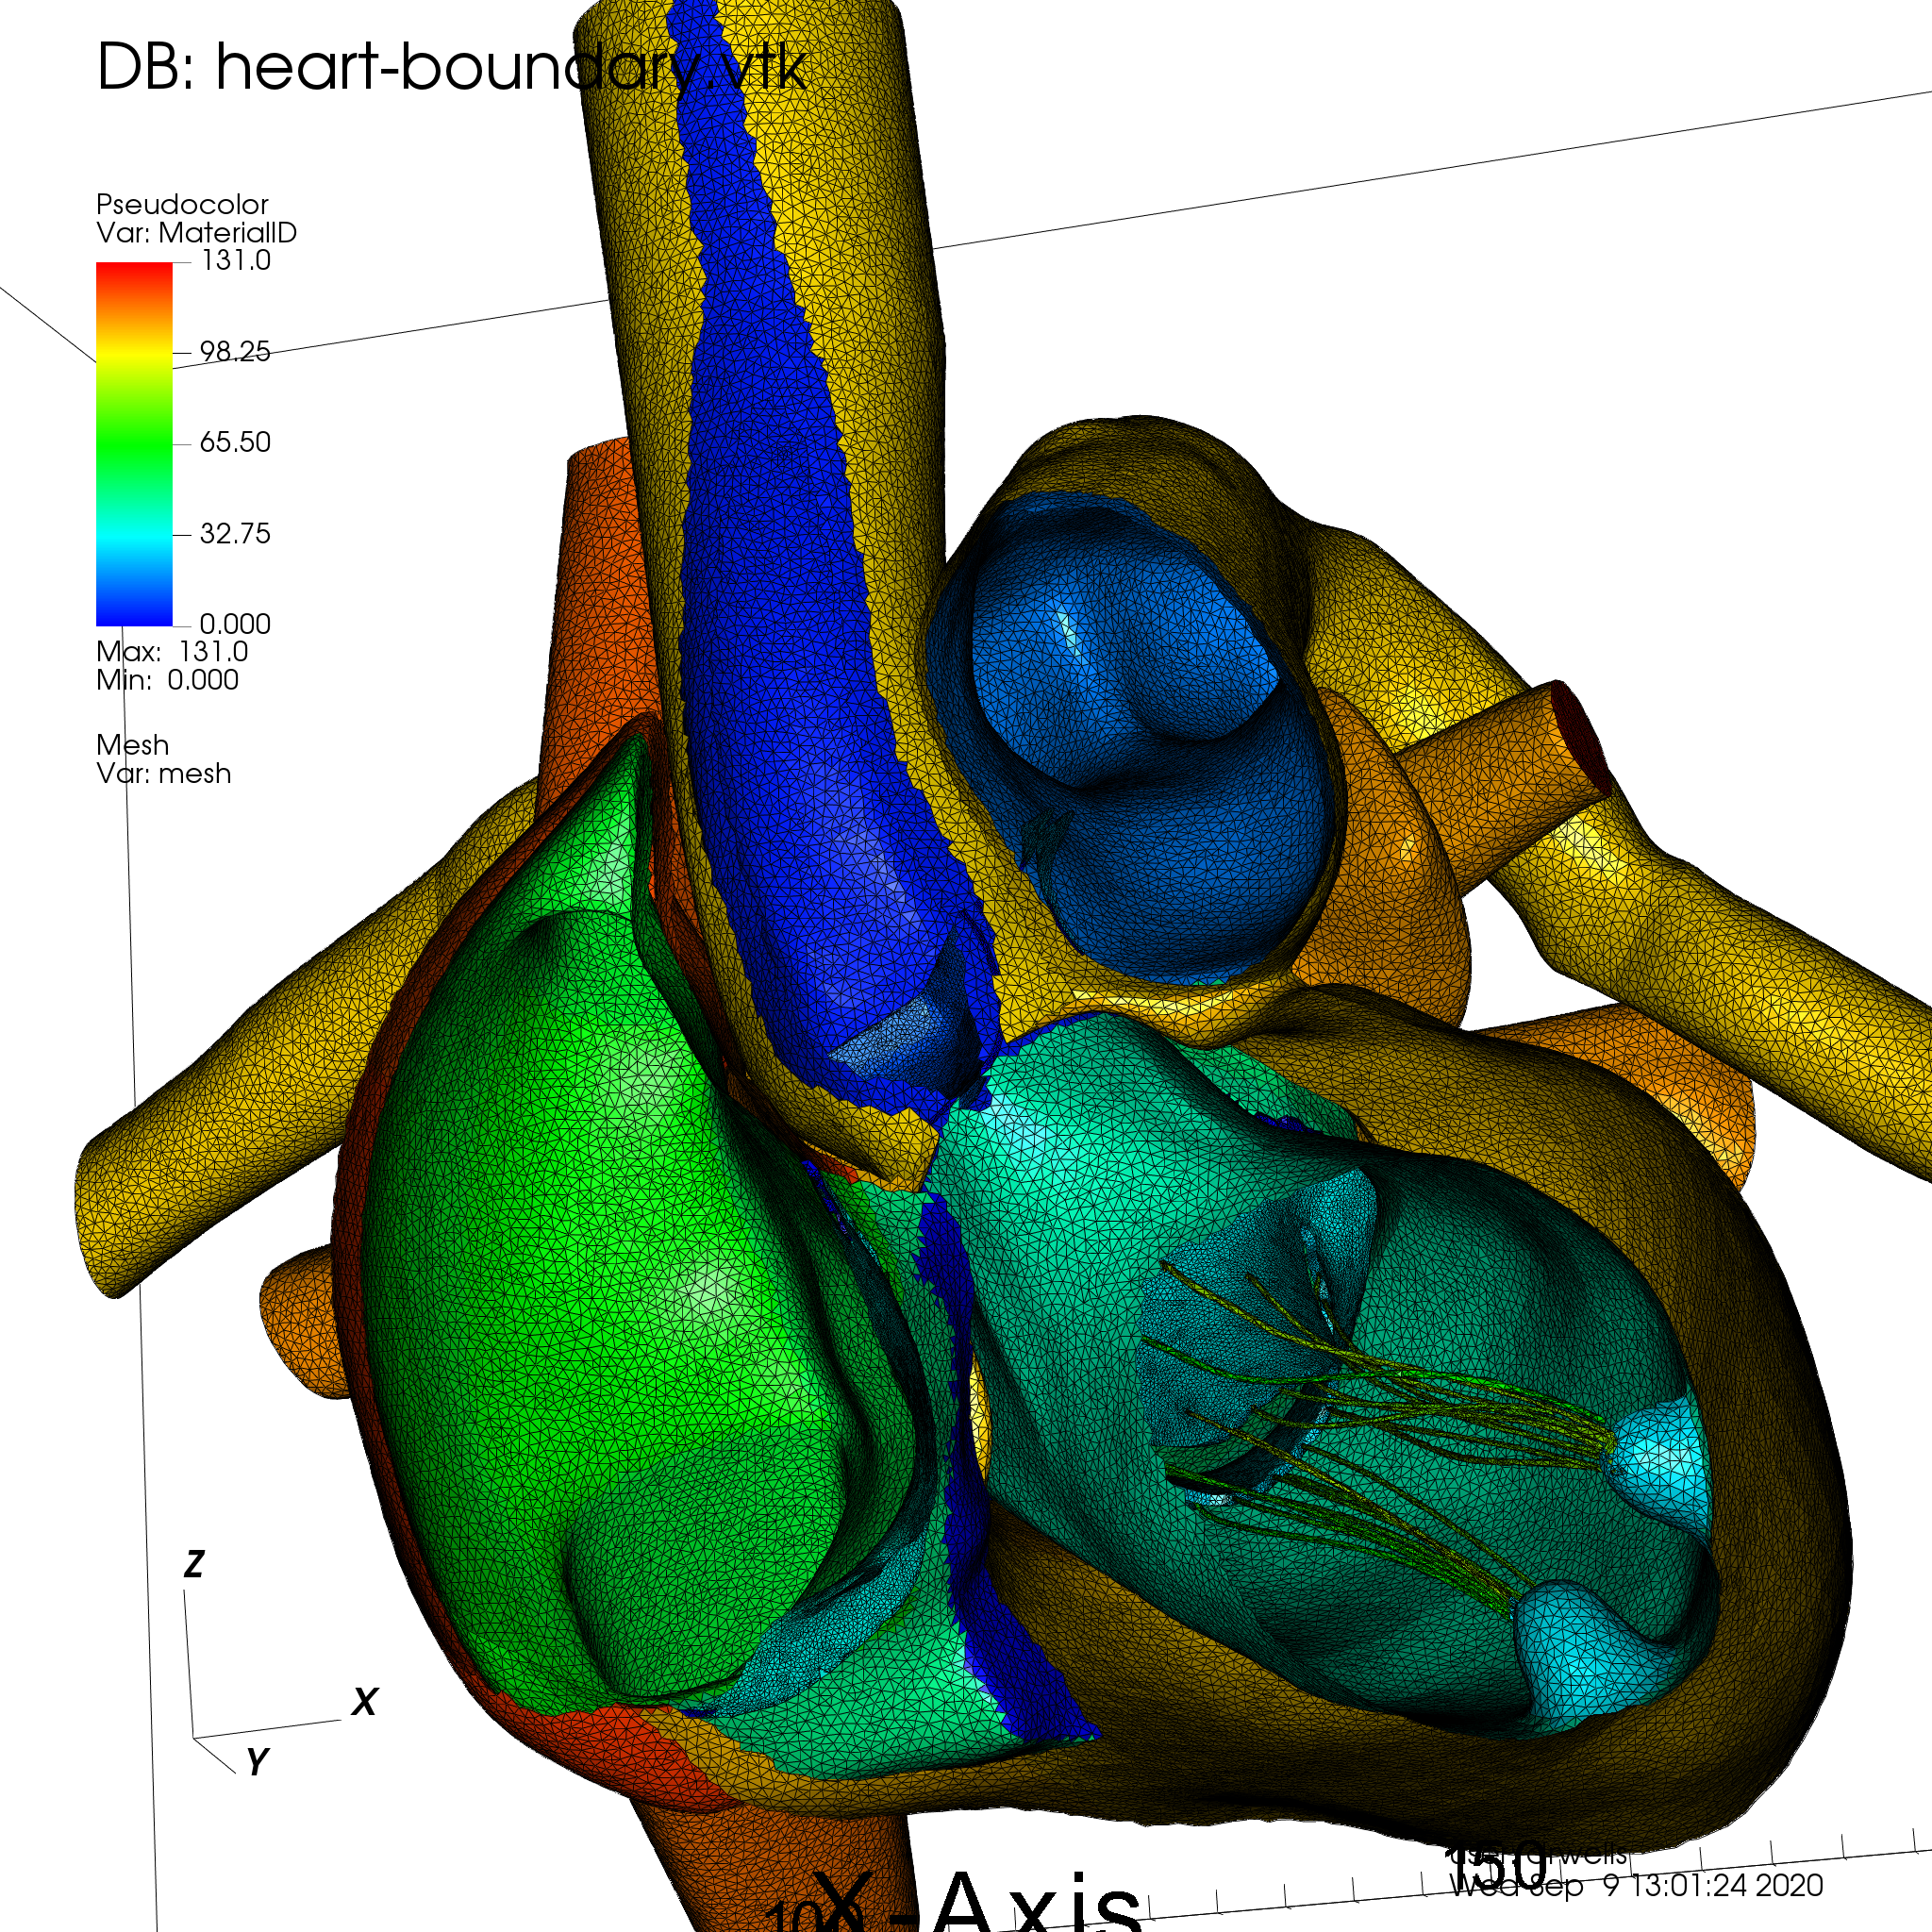
\includegraphics[width=2.5in]{heartmesh2.png}
    \end{figure}
    25 forces or stresses, 9 active strain models, electrophysiology (Abdala)
    and mechanics (Davey) - come to Boyce's talk!
\end{frame}

\section{Fluid-Structure Interaction}
\begin{frame}
    \frametitle{Partitioned and monolithic methods}
    \begin{itemize}
        \item[$\blacksquare$] \emph{monolithic scheme}: fluid and structure are
        coupled in one algebraic system (solve for everything simultaneously)
        \item[$\blacksquare$] \emph{partitioned scheme}: stagger fluid and
        structure solves (do a fluid step then a structure step)
    \end{itemize}
    \vfill
    Advantages of partitioned methods:
    \begin{itemize}
        \item[$\blacksquare$] code reuse (moving from libMesh to deal.II
          without modifying IBAMR)
        \item[$\blacksquare$] different algorithms for different domains (FDM and FEM)
    \end{itemize}
    primary disadvantage: difficult numerical instabilities
\end{frame}

\begin{frame}
  \frametitle{The Added-Mass Instability}
    The traditional coupling scheme:
    no-slip boundary condition (structure to fluid), normal force given by
    traction (fluid to structure). Works well for aircraft. This ignores the
    work needed to move the fluid out of the structure's way.

    \begin{center}
        
\includegraphics[width=1.80in]{left.png}
        \hspace{0.5in}
        
\includegraphics[width=1.80in]{right.png}
    \end{center}
\end{frame}

\begin{frame}
    \frametitle{The Immersed Boundary Method}
    \begin{figure}
        \centering
        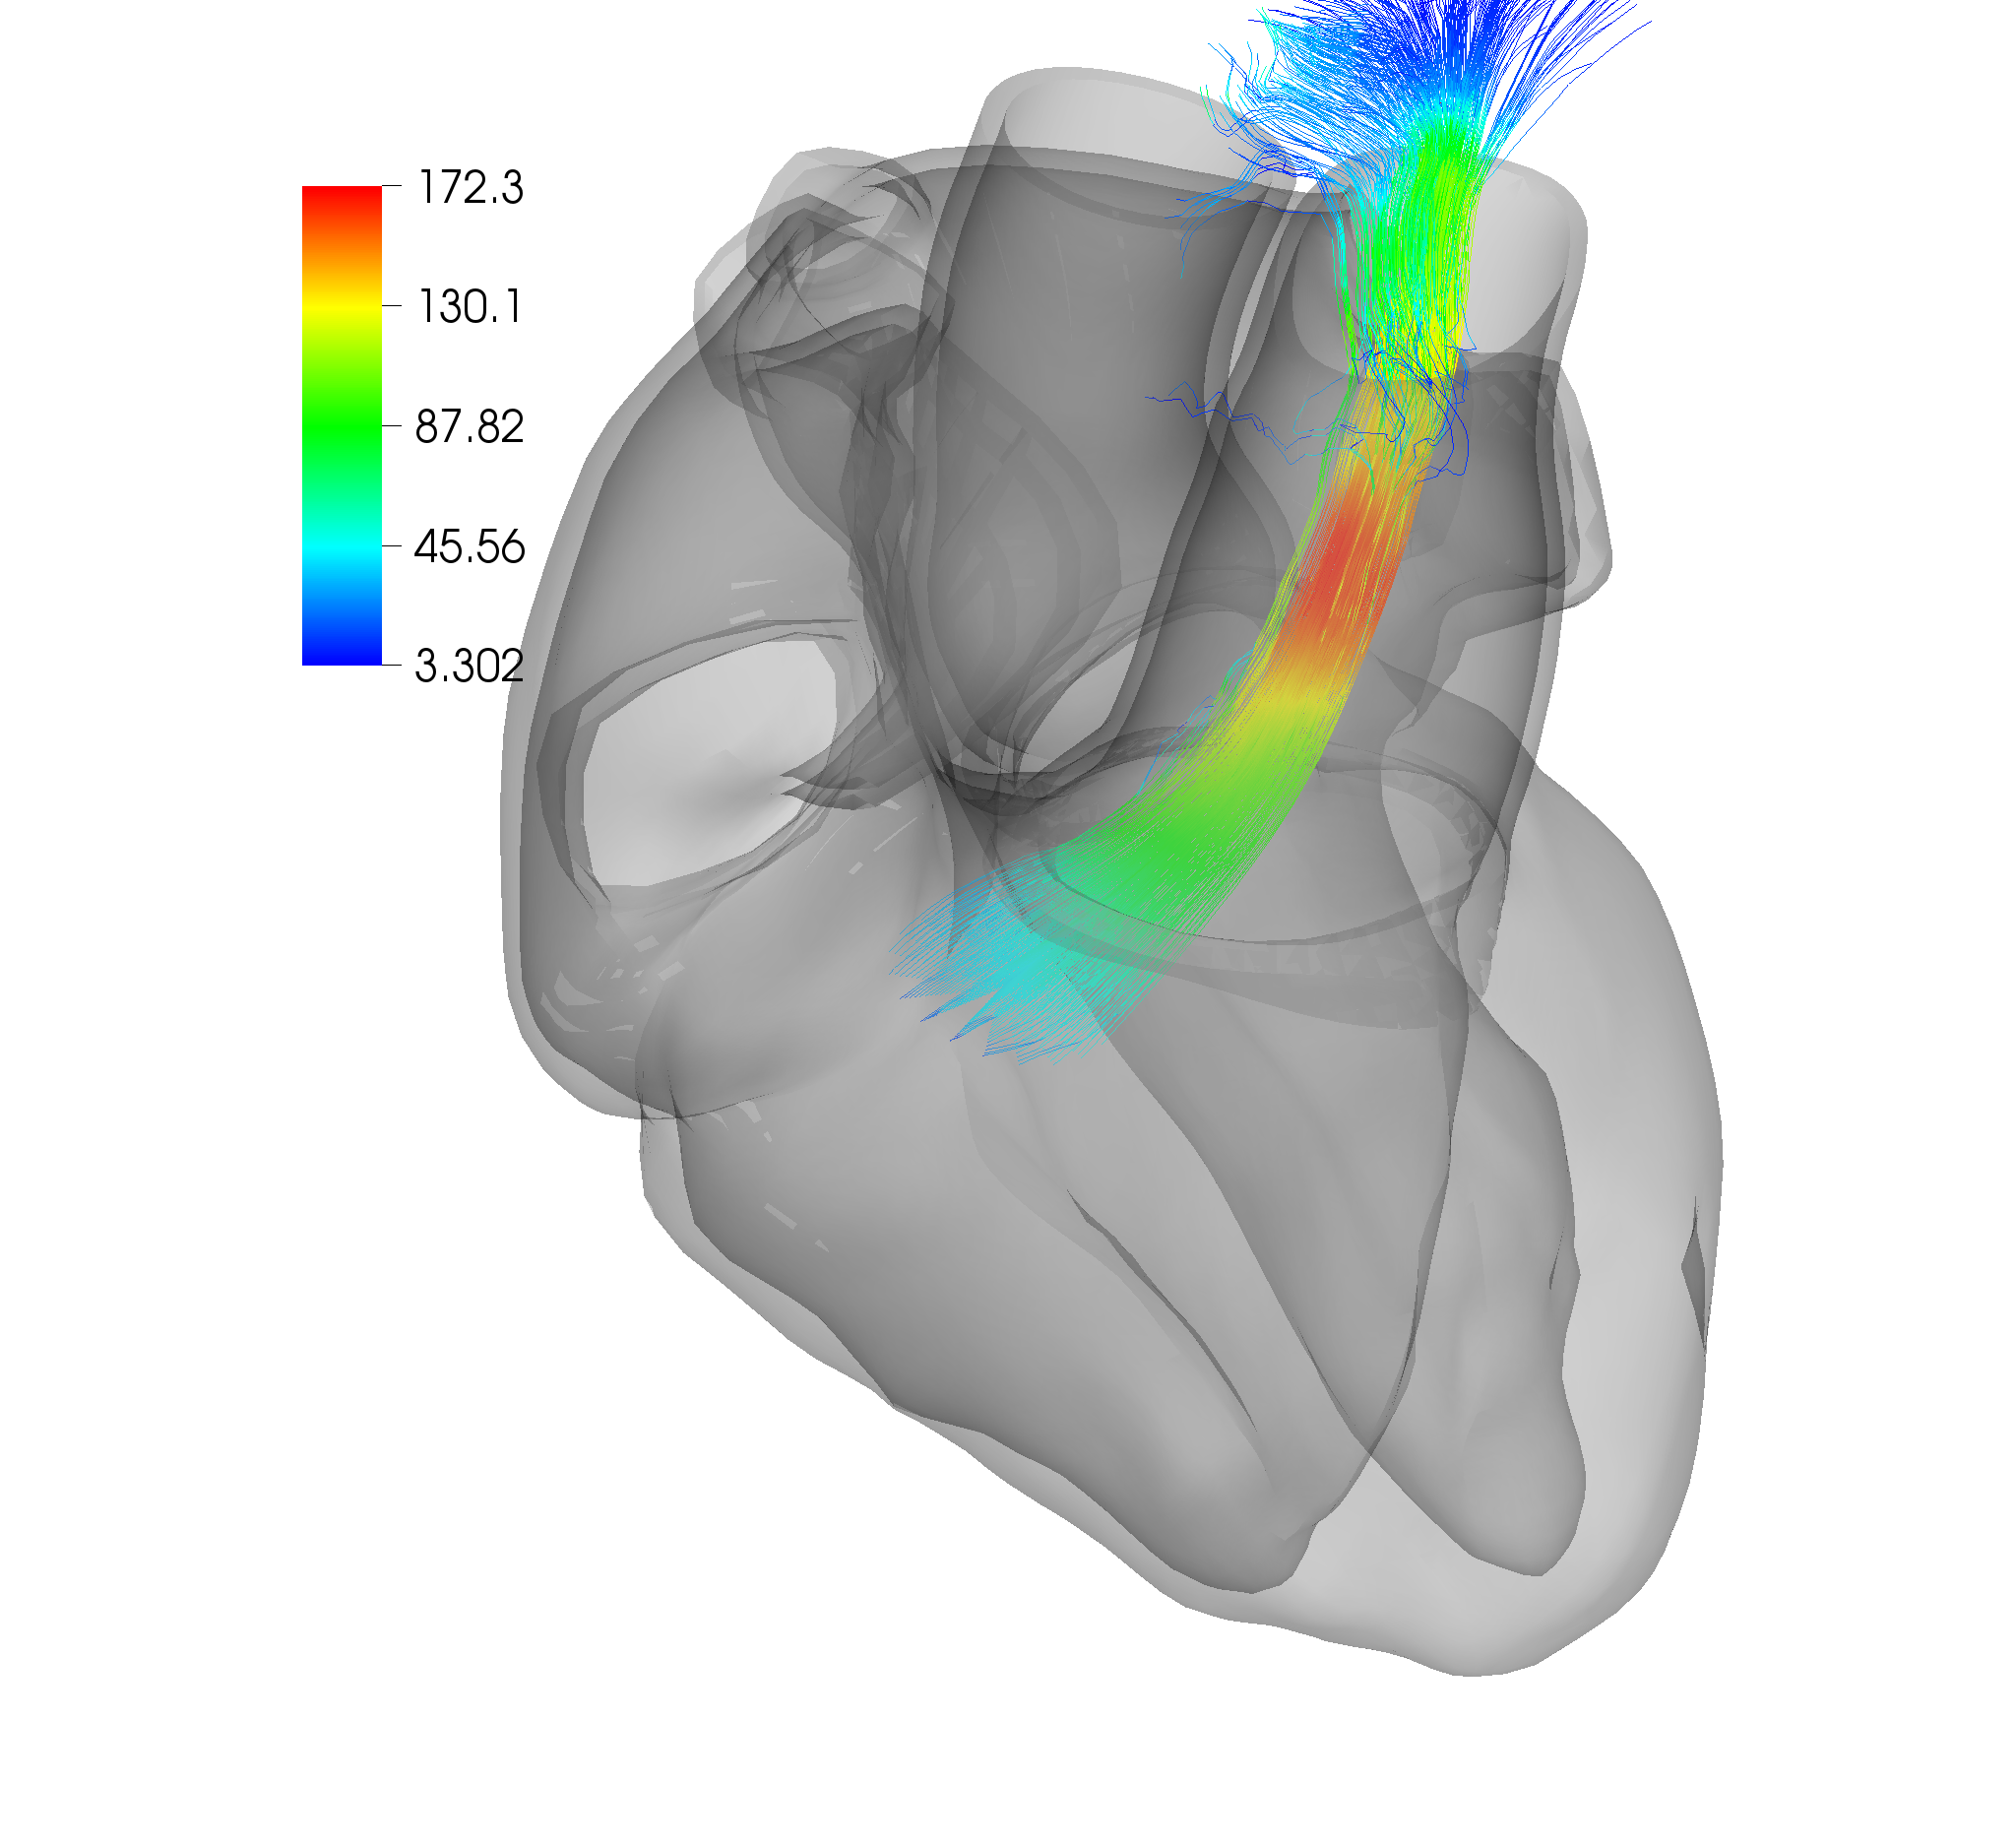
\includegraphics[width=2in]{vel_streamlines_RV.png}
    \end{figure}
    \begin{itemize}
        \item[$\blacksquare$] Solve for the fluid at all points (\emph{including
        inside the structure})
        \item[$\blacksquare$] Structure velocity given by fluid velocity
        \item[$\blacksquare$] Fluid force is given by the structure force
        density
        \item[$\blacksquare$] Coupling is done by regularized delta functions
        (\(\delta_h\))
    \end{itemize}
\end{frame}

\begin{frame}
    \frametitle{The Immersed Boundary Method}
    \begin{figure}
        \centering
        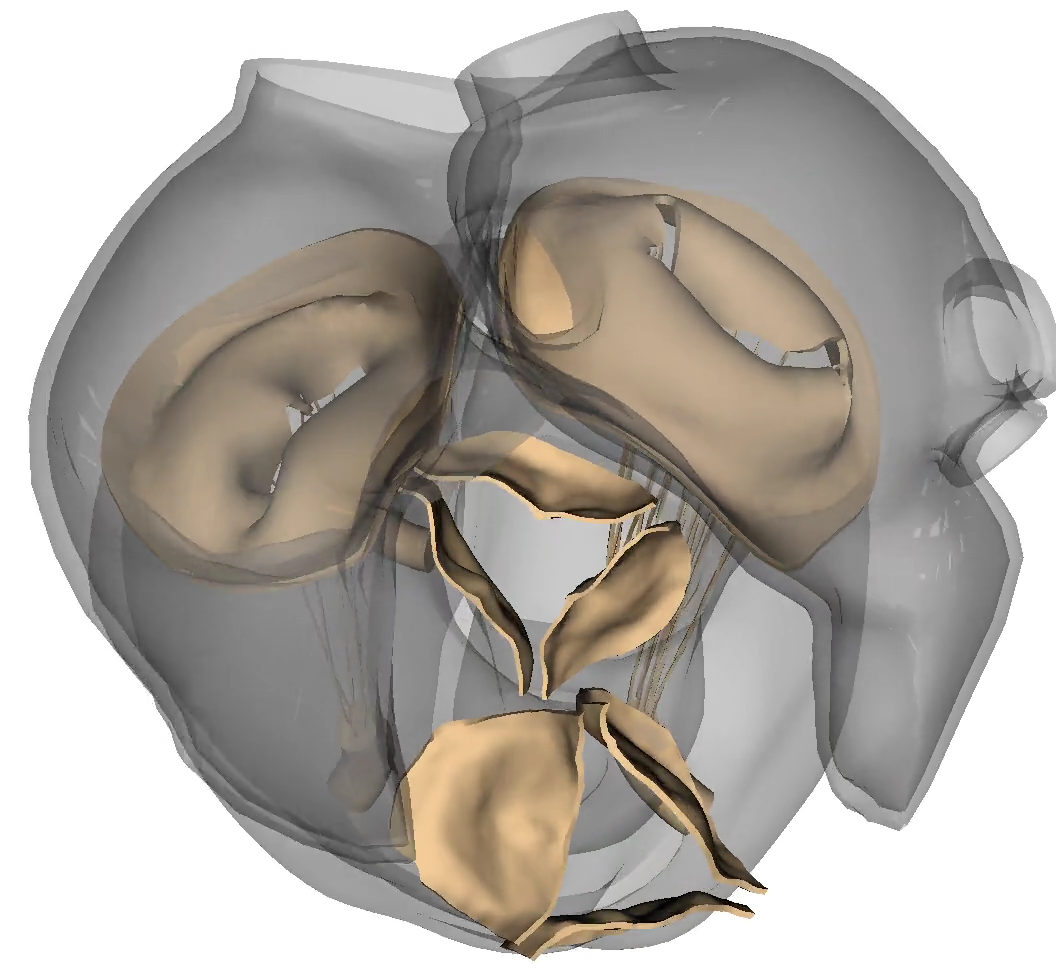
\includegraphics[width=1.5in]{mov3_Guccione0032.png}
    \end{figure}
    Advantages:
    \begin{itemize}
        \item[$\blacksquare$] Partitioned method
        \item[$\blacksquare$] Works well with really hard geometries
        \item[$\blacksquare$] Cartesian fluid domain
        \item[$\blacksquare$] coupling (velocity projection, force spreading)
        are adjoint operators: conserve force, torque
    \end{itemize}
    Disadvantages:
    \begin{itemize}
        \item[$\blacksquare$] First order velocity convergence at
        fluid-structure boundaries (fix: \emph{Immersed Interface Method},
        Ebrahim Kolahdouz)
        \item[$\blacksquare$] Coupling occurs across a volume, not an interface
        (alleviated by nodal coupling, see the 2024 paper)
    \end{itemize}
\end{frame}

\begin{frame}
    \frametitle{The Immersed Boundary Method}
    \begin{align*}
        \rho
        \left(
        \dfrac{\partial\mathbf{u}(\xb, t)}{\partial t}
        + \mathbf{u}(\xb, t) \cdot \nabla \mathbf{u}(\xb, t)
        \right)
        &= -\nabla p(\xb, t)
        + \mu \Delta \mathbf{u} (\xb, t)
        + \mathbf{f}(\xb, t),                                          \\
        \nabla \cdot \mathbf{u}(\xb, t) &= 0,                          \\
        \dfrac{\partial \Chib(\Xb, t)}{\partial t} &=
        \mathbf{u}(\Chib(\Xb, t), t)
        = \int_\Omega \mathbf{u}(\xb, t)
        \delta (\xb - \Chib(\Xb, t)) d\xb,                \\
        \mathbf{f}(\xb, t) &=
        \int_\Omega \mathbf{F}(\Xb, t)
        \delta(\xb - \Chib(\Xb, t)) d\Xb,                 \\
        \int_\Omega \mathbf{F}(\Xb, t) \cdot \phi(\Xb) d\Xb
        &= -\int_\Omega \dfrac{\partial W}{\partial \Xb} : \nabla_{\Xb}
        \phi(\Xb) d\Xb, \forall \phi \in X^h(\Omega)
    \end{align*}
    lower case variables are Eulerian, upper case are Lagrangian. Integration by parts actually removes a surface integral.
\end{frame}

\begin{frame}
    \frametitle{Fluid to structure: velocity projection}
    \begin{figure}
        \includegraphics[width=2in]{ibcoupling.pdf}
    \end{figure}
    \begin{align*}
        \dfrac{\partial}{\partial t} \Chib(\Xb, t)
        &= \mathbf{U}(\Xb, t) \text{ where}                            \\
        \int_U \mathbf{U}(\Xb, t) \phi(\Xb) d\Xb &=
        \int_U \mathbf{V}(\Xb, t) \phi(\Xb) d\Xb, \forall
        \phi \in X^h(\Omega)                                           \\
        \mathbf{V}(\Xb, t) &= \sum_{i,j,k} \mathbf{u}_{i,j,k}
        \delta_h(\xb_{i,j,k} - \Chib(\Xb, t))
        \Delta \xb^3
    \end{align*}
\end{frame}

\begin{frame}
    \frametitle{Structure to fluid: force spreading}
    \begin{figure}
        \includegraphics[width=2in]{ibcoupling.pdf}
    \end{figure}
    \begin{align*}
        \mathbf{f}(\xb_{i,j,k}, t) &=
        \int_U \mathbf{F}(\Xb, t)
        \delta_h(\xb_{i,j,k} - \Chib(\Xb, t))
        d\Xb                                                          \\
    \end{align*}
    Here \(-\mathbf{F}\) is the FE projection of the structural stress tensor (a
    force density). Comes from material models of heart tissue.
\end{frame}

\section{Where do we use PETSc?}
\begin{frame}[fragile]
    \frametitle{All our fluid solvers are \texttt{KSP}s}
    \vfill
    \begin{itemize}
      \item[$\blacksquare$] Wrap SAMRAI data as
        \texttt{IBTK::PETScSAMRAIVectorReal}, which is a \texttt{Vec}
        \vfill
      \item[$\blacksquare$] Wrap solvers as
        \texttt{IBTK::PETScKrylovLinearSolver}, which has \texttt{Mat}s
        and \texttt{KSP}s
        \vfill
      \item[$\blacksquare$] SAMRAI and \texttt{MatShell}: lots of
        \texttt{FORTRAN 77} loops over structured grid data
        \vfill
      \item[$\blacksquare$] Command-line flags are really helpful!
        \begin{verbatim}
mpiexec ./main3d full-heart.input   \
 -stokes_ksp_error_if_not_converged \
 -stokes_ksp_monitor                \
 -velocity_ksp_type cg              \
 -velocity_pc_type none             \
 -velocity_ksp_norm_type none       \
 -pressure_ksp_norm_type none       \
 -stokes_ksp_rtol 1.0e-6            \
 -stokes_ksp_converged_reason
        \end{verbatim}
    \end{itemize}
    \vfill
\end{frame}

\begin{frame}
    \frametitle{Force spreading}
    \vfill
    \begin{align*}
      \mathbf{f}(\xb, t)
        &= \int_\Omega \mathbf{F}(\Xb, t) \\
        f^1_{\xface}
        &= \sum_{(\Xb_q, w_q) \in \mathbb{Q}_q} F^1(\Xb_{q})
          \, \delta_h(\xb_{\xface} - \Chib_h(\Xb_{q}))w_{q}
    \end{align*}
    \vfill
    This is like computing a load vector: each $f^1_{\xface}$ has
    contributions from adjacent (by width of $\delta_h$) quadrature points.
    \vfill
\end{frame}

\begin{frame}
    \frametitle{Force spreading}
    Still need to associate (in parallel) elements with patches (load balanced for the quadrature points).
        \vfill
    \begin{itemize}
      \item[$\blacksquare$] Prototype: consider quadrature points which spread into a Patch (i.e., a ghost region wide enough to cover $\delta_h$)
        \vfill
      \item[$\blacksquare$] Enhancement: loop over all quadrature points are inside a patch (25\% fewer, can load balance on the number of quadrature points)
    \end{itemize}

    \vfill
    Implemented in IBAMR as \texttt{IBTK::SAMRAIGhostDataAccumulator}.
\end{frame}

\begin{frame}
    \frametitle{Force spreading}
    \vfill
    Represent Eulerian force values with a \texttt{VECGHOST}:
    \begin{itemize}
      \item[$\blacksquare$] $O(\mathrm{nproc})$ patches, known globally
      \item[$\blacksquare$] Relatively easy to enumerate the DoFs and ghost DoFs
      \item[$\blacksquare$] Nonphysical DoFs (outside domains) are \texttt{-1}s
        (nice feature!)
    \end{itemize}
    \vfill
    Global indices are slow, local indices are fast
    \begin{itemize}
      \item[$\blacksquare$] \texttt{VecGetLocalToGlobalMapping()} and \texttt{ISGlobalToLocalMappingApply()} (and store with SAMRAI)
      \item[$\blacksquare$] \texttt{VecGhostGetLocalForm()}, \texttt{VecSetValues()}, \texttt{VecGhostRestoreLocalForm()}
      \item[$\blacksquare$] \texttt{VecGhostUpdateBegin()}, \texttt{VecGhostUpdateEnd()} (\texttt{PetscSF} is good)
      \item[$\blacksquare$] Done!
    \end{itemize}
    \vfill
\end{frame}

\begin{frame}
    \frametitle{Velocity interpolation}
    \vfill
    \begin{align*}
        \mathbf{u}(\Chib(\Xb, t), t)
        &= \int_\Omega \mathbf{u}(\xb, t)
        \delta (\xb - \Chib(\Xb, t)) d\xb                \\
        U^{\text{IB},1}(\Xb_q) &= \sum_{i,j,k} u^1_{\xface}
        \, \delta_h(\xb_{\xface} - \Chib_h(\Xb_q)) \euleriandx^3 \\
        \int \phi \cdot \mathbf{U}^h d\Xb
        &= \int \phi \cdot \mathbf{U}^{\text{IB}} d\Xb, \forall \phi \in X^h(\Omega)
    \end{align*}
    \vfill
    Adjoint of of force spreading - we need to accumulate a finite element load vector this time.
    \vfill
\end{frame}

\begin{frame}
    \frametitle{Velocity interpolation}

    \begin{itemize}
      \item[$\blacksquare$] Prototype: Ignore problem, libMesh stores all DoFs
        on every processor, use \texttt{VecStash} (works, but slow)
      \item[$\blacksquare$] Enhanced: Same global DoF ordering for libMesh,
        ghost region based on which elements intersect local patches. Set up
        proper ghost regions with \texttt{VECGHOST} (as an FE vector this time!)
      \item[$\blacksquare$] More Enhanced: deal.II now has fully distributed tet
        meshes, use those and deal.II's version of \texttt{VecScatter}/\texttt{PetscSF}
        (\texttt{dealii::MPI::Partitioner} and \texttt{Cardinal::Scatter})
    \end{itemize}
\end{frame}

\section{Future Work}
\begin{frame}[fragile]
    \frametitle{Numerical stiffness in explicit IB methods}

    The heart model is pretty far from $\Delta x = \Delta t$:
    \begin{verbatim}
// Solver parameters
IB_DELTA_FUNCTION   = "BSPLINE_3"
SOLVER_TYPE         = "STAGGERED"
DT                  = 0.0000625*DX/2.0
START_TIME          = 0.0
END_TIME            = 1.049
    \end{verbatim}
    Explicit treatment of forces
    \begin{equation*}
        \int_\Omega \mathbf{F}(\Xb, t) \cdot \phi(\Xb) d\Xb
        = -\int_\Omega \dfrac{\partial W}{\partial \Xb} : \nabla_{\Xb}
        \phi(\Xb) d\Xb, \forall \phi \in X^h(\Omega)
    \end{equation*}
    doesn't work well for very stiff objects (chordae, penalty forces, very
    stiff biological materials, steel, etc.).

    \vfill
    \emph{Fix}: New method (Gruninger) makes implicit timestepping work without
    introducing nonlinearities. Boyce and I need help implementing with
    \texttt{PCPATCH}.
\end{frame}

\begin{frame}
    \frametitle{Cardinal}

    Students encounter a lot of similar problems in their PhDs:
    \vfill
    \begin{itemize}
      \item[$\blacksquare$] Compiling stuff (autoibamr)
        \vfill
      \item[$\blacksquare$] Learning how to code, use clusters, etc.
        \vfill
      \item[$\blacksquare$] Learning how to manage projects, complexity
        \vfill
      \item[$\blacksquare$] Postprocessing, visualization, statistics
        \vfill
      \item[$\blacksquare$] Canonical implementations of material and electrical
        models (public versions have bugs)
        \vfill
    \end{itemize}

    Students need to learn these skills, but they shouldn't have to start from
    scratch. Most IBAMR apps are pretty similar!
\end{frame}

\begin{frame}
    \frametitle{Cardinal}

    Cardinal is a (closed-course for now) IBAMR app driven by plugins and input
    files.
    \vfill
    \begin{itemize}
      \item[$\blacksquare$] Heart model input file is 800 lines long: too much
        for command line arguments
      \item[$\blacksquare$] We should centralize \texttt{main()} so that everyone gets
        all algorithmic improvements
      \item[$\blacksquare$] Centralized IO facilities (one HDF5 file, not a dozen
        text files): how do PETSc people log lots of quantities?
      \item[$\blacksquare$] WIP: semiexplicit mechanics models, managed with
        \texttt{TS}, operator splitting, coupling with IB methods
    \end{itemize}
\end{frame}

\end{document}
